\documentclass[border=10pt]{standalone}
\usepackage{xcolor}
\usepackage{tikz}
\usepackage{pgfplots}
\pgfplotsset{compat=1.18}
\usetikzlibrary{arrows.meta}

\definecolor{BG}{HTML}{FAFAFA}
\definecolor{INK}{HTML}{1A1A2E}
\definecolor{SUB}{HTML}{555566}
\definecolor{COLD}{HTML}{4361EE}
\definecolor{WARM}{HTML}{2EC4B6}
\definecolor{NEW}{HTML}{F4A261}

\begin{document}
\pagecolor{BG}
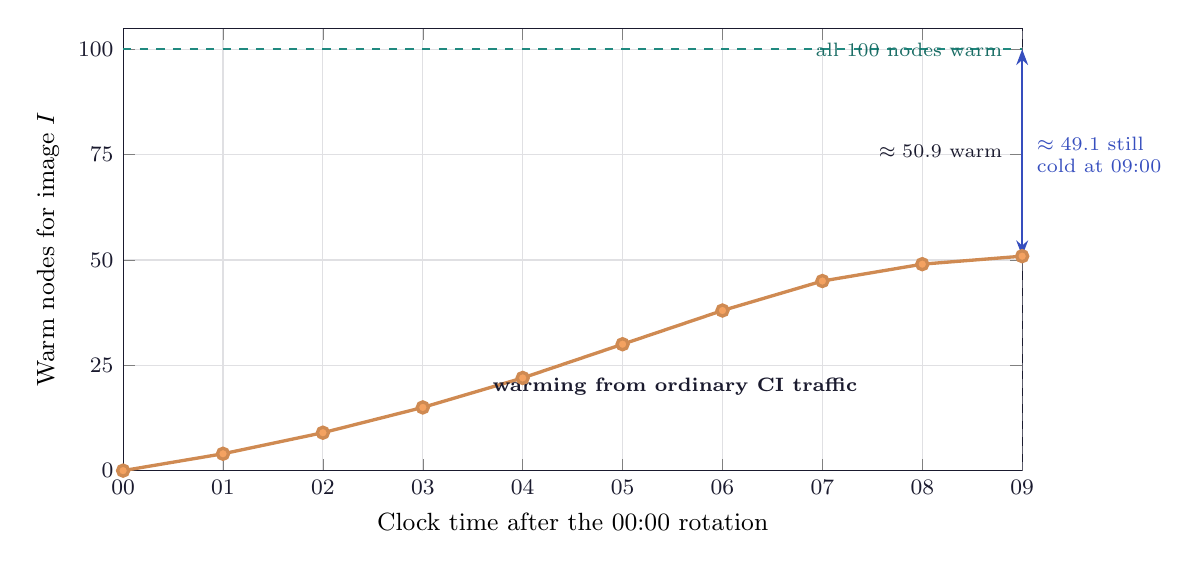
\begin{tikzpicture}[font=\sffamily]
\begin{axis}[
  width=13cm, height=7.2cm,
  xlabel={Clock time after the 00:00 rotation},
  ylabel={Warm nodes for image \(I\)},
  xmin=0, xmax=9, ymin=0, ymax=105,
  xtick={0,1,2,3,4,5,6,7,8,9},
  xticklabels={00,01,02,03,04,05,06,07,08,09},
  ytick={0,25,50,75,100},
  axis line style={INK},
  every axis label={INK},
  tick label style={INK, font=\footnotesize},
  label style={font=\small},
  grid=major, grid style={SUB!18},
  clip=false,
]
% all-nodes reference
\addplot[dashed, thick, WARM!70!black, mark=none] coordinates {(0,100) (9,100)};
\node[anchor=east, font=\scriptsize, text=WARM!55!black] at (axis cs:8.9,100) {all 100 nodes warm};

% warming curve from background traffic (~50.9 warm by 09:00)
\addplot[very thick, NEW!85!black, mark=*, mark options={fill=NEW}] coordinates {
  (0,0) (1,4) (2,9) (3,15) (4,22) (5,30) (6,38) (7,45) (8,49) (9,50.9)
};

% dev window boundary
\draw[dashed, INK!70] (axis cs:9,0) -- (axis cs:9,105);
\node[anchor=south east, font=\scriptsize, text=INK] at (axis cs:8.9,72)
  {\(\approx 50.9\) warm};
\draw[COLD!80!black, {Stealth[length=2mm]}-{Stealth[length=2mm]}, thick]
  (axis cs:9,50.9) -- (axis cs:9,100);
\node[anchor=west, font=\scriptsize, text=COLD!80!black, align=left] at (axis cs:9.05,75)
  {\(\approx 49.1\) still\\cold at 09:00};
\node[anchor=west, font=\scriptsize\bfseries, text=INK] at (axis cs:3.6,20)
  {warming from ordinary CI traffic};
\end{axis}
\end{tikzpicture}
\end{document}
